\subsection{Maquette}
\begin{figure}[H]
    \begin{center}
        \frame{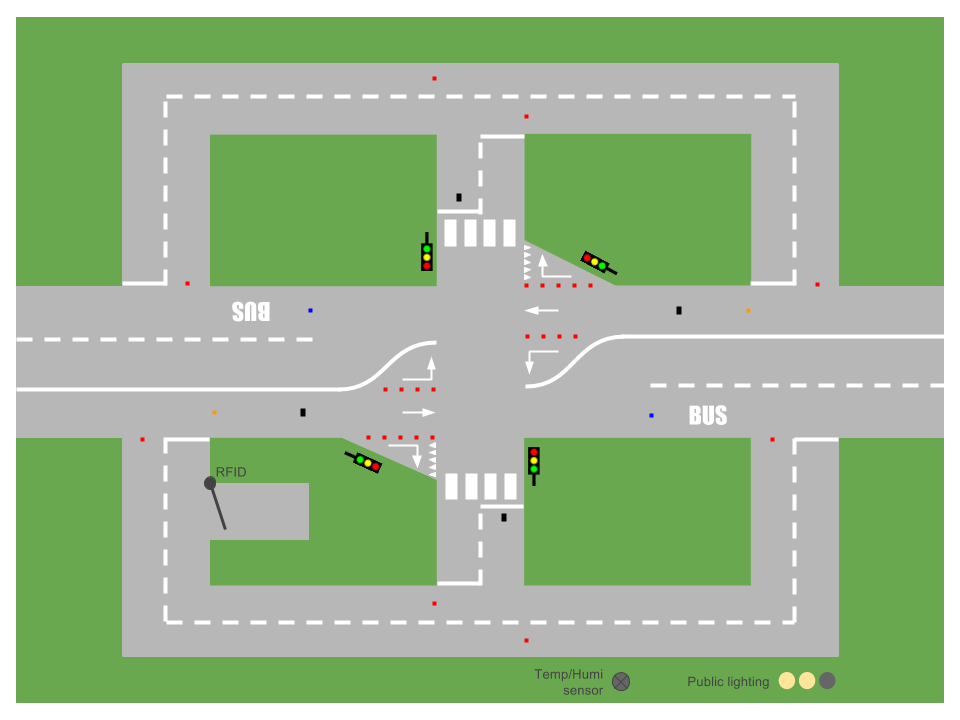
\includegraphics[width=\linewidth, height=\textheight,keepaspectratio]{img/maquette}}

        \caption{Croquis de la maquette}\label{croquis-maquette}
    \end{center}
\end{figure}
\vspace{-0.7cm}
Afin de pouvoir utiliser les senseurs de manière optimale, nous avons imaginé la maquette telle que ci-dessus (illustration \ref{croquis-maquette}). Les LEDs rouges représentent des interdictions. Lorsqu’elles sont allumées, les automobilistes ne peuvent pas aller dans ces rues. Les deux LEDs bleues sont pour les bandes de bus. Allumées, elles indiquent que la bande est réservée aux bus, et donc que les autres usagers doivent tous se rabattre sur la seconde bande. Le RFID est utilisé comme entrée d’un parking (ici, dans la partie inférieure gauche de la maquette).
